% !TeX root = b01.tex

\documentclass[
    a4paper,
    12pt,
]{article}

\usepackage[
    top=3cm,
    bottom=3cm,
    left=2.5cm,
    right=2.5cm
]{geometry}

\usepackage[T1]{fontenc}
\usepackage[utf8]{inputenc}
\usepackage[ngerman]{babel}

\setcounter{secnumdepth}{0}

\usepackage{parskip}

\usepackage[
  final,
  colorlinks=true,
  linkcolor=blue
]{hyperref}
\usepackage[htt]{hyphenat}  % htt -> allow to hyphenate TT text

\usepackage{multirow}
\usepackage{amsmath}
\usepackage{amssymb}

\usepackage{graphicx}
\usepackage{subfig}
\usepackage{caption,subcaption}
\usepackage{float}

\usepackage{csquotes}
\usepackage{amsbsy} % bold maths symbols, \bm{} or \pmb{}

\usepackage{fancyhdr}

\usepackage[many]{tcolorbox}
\newtcolorbox{task}{
    enhanced,
    boxrule = 0pt,
    frame hidden,
    borderline west = {0.5mm}{0.0mm}{black},
    breakable,
}

% https://tex.stackexchange.com/questions/24186/#24197
\newenvironment{tightcenter}{%
  \setlength\topsep{0pt}
  \setlength\parskip{0pt}
  \begin{center}
}{%
  \end{center}
}

% vertical padding in tables
\renewcommand{\arraystretch}{1.2}


\newcommand{\maintitle}{Beleg 1}
\newcommand{\topic}{Beschreibende Statistik}
\newcommand{\theauthor}{Nico Schramm}
\newcommand{\module}{Empirische Methoden für Informatiker}
\newcommand{\shortmodule}{EMI}
\newcommand{\uni}{HTWK Leipzig}
\date{\today}

\title{%
    \maintitle \\
    \large \topic \\
    \module}
\author{\theauthor}

\hypersetup{
    pdfauthor={\theauthor},
    pdftitle={\maintitle\space(\shortmodule)},
    pdfsubject={\topic}
}

\pagestyle{fancy}
\fancyhead[L]{\maintitle}
\fancyhead[R]{\module}
\fancyfoot[L]{\theauthor}
\fancyfoot[C]{\thepage}
\fancyfoot[R]{\uni}


\begin{document}

\maketitle
\tableofcontents

% !TeX root = ../b01.tex

\section{Aufgabe BI-1}

\begin{task}
    Die Pizzeria \textsc{Morte Dolce} (des Eigentümers \textsc{M.A. Fia}) hat zwei Lokale (kurz L1 und L2 genannt), bei denen man Mittag- und Abendessen (kur M und A) einnehmen kann, wobei es jedoch bei den Gerichten jeweils nur grob die Unterteilung zwischen Pizza, Spaghetti, Ravioli und Canneloni gibt. Im letzten Monat (September) wurden in jener Pizzeria wie folgt Gericht bestellt, aufgetischt und verspeist:

    \begin{table}[H]
    \centering
    \begin{tabular}{l||cc|cc||c}
        \multirow{2}{*}{} & \multicolumn{2}{c|}{\bf{L1}}  & \multicolumn{2}{c||}{\bf{L2}} &                         \\
                          & \multicolumn{1}{c}{M}         & A    & \multicolumn{1}{c}{M}  & A           & insgesamt \\ \hline\hline
        Pizza             & \multicolumn{1}{c}{400}       & 600  & 600                    & 800         & 2400      \\
        Sonstige          & \multicolumn{1}{c}{700}       & 1100 & 400                    & 400         & 2600      \\
        Summe             & \multicolumn{1}{c}{1100}      & 1700 & 1000                   & 1200        & 5000     
    \end{tabular}
    \end{table}

    \begin{enumerate}
        \item[(a)] Wie viele Merkmale werden in dieser Tabelle dargestellt, wie heißen diese und welche Merkmalsausprägungen werden hierbei jeweils berücksichtigt?
    \end{enumerate}
\end{task}

\begin{task}
    \begin{enumerate}
        \item[(b)] Was (Grundgesamtheit, statistische Einheit, Merkmal usw.) stellt im Falle dieser Datenerhebung jeweils das folgende dar:
        \begin{enumerate}
            \item[($b_1$)] die Angabe L2?
            \item[($b_2$)] Herr \textsc{M. Angione}, der am 1. September mittags in L1 Canneloni gegessen hat?
            \item[($b_3$)] die Zahl 5000?
            \item[($b_4$)] die 2400 Leute, denen eine Pizza aufgetischt wurde?
        \end{enumerate}
    \end{enumerate}
\end{task}

% !TeX root = ../b01.tex

\section{Aufgabe BI-2}

\begin{task}
    Für die Bevölkerung gewisser Regionen der Erde wurden folgende Geschlechterverteilungen (das heißt Männer 100 Frauen):
    \begin{tightcenter}
        96  101  98  96  101  98  105  106  101  104  88  97 \\
        100  96  101  92  98  104  102  97  98  93  100  94
    \end{tightcenter}
    durch statistische Erhebungen erhalten.

    \begin{enumerate}
        \item[(a)] Stellen Sie die Daten in einem Histogramm mit 5 Klassen gleicher Klassenbreite dar.
    \end{enumerate}
\end{task}

\begin{task}
    \begin{enumerate}
        \item[(b)] Berechnen Sie die Werte der (gewöhnlichen, nicht klassierten) empirischen Verteilungsfunktion $F$ der Daten an den Stellen $x_1=95.5$ und $x_2=100$.
    \end{enumerate}
\end{task}

\begin{task}
    \begin{enumerate}
        \item[(c)] Erstellen Sie den zu den Beobachtungswerten gehörigen klassischen Box-Plot (mit Kennzeichnung von Ausreißern und Extremwerten, so vorhanden).
    \end{enumerate}
\end{task}

% !TeX root = ../b01.tex

\section{Aufgabe BI-3}

\begin{task}
    Die folgende Graphik zeigt für $n=200$ Beobachtungen eines Merkmals $X$ die empirische Verteilungsfunktion:

    \begin{figure}[H]
        \begin{center}
            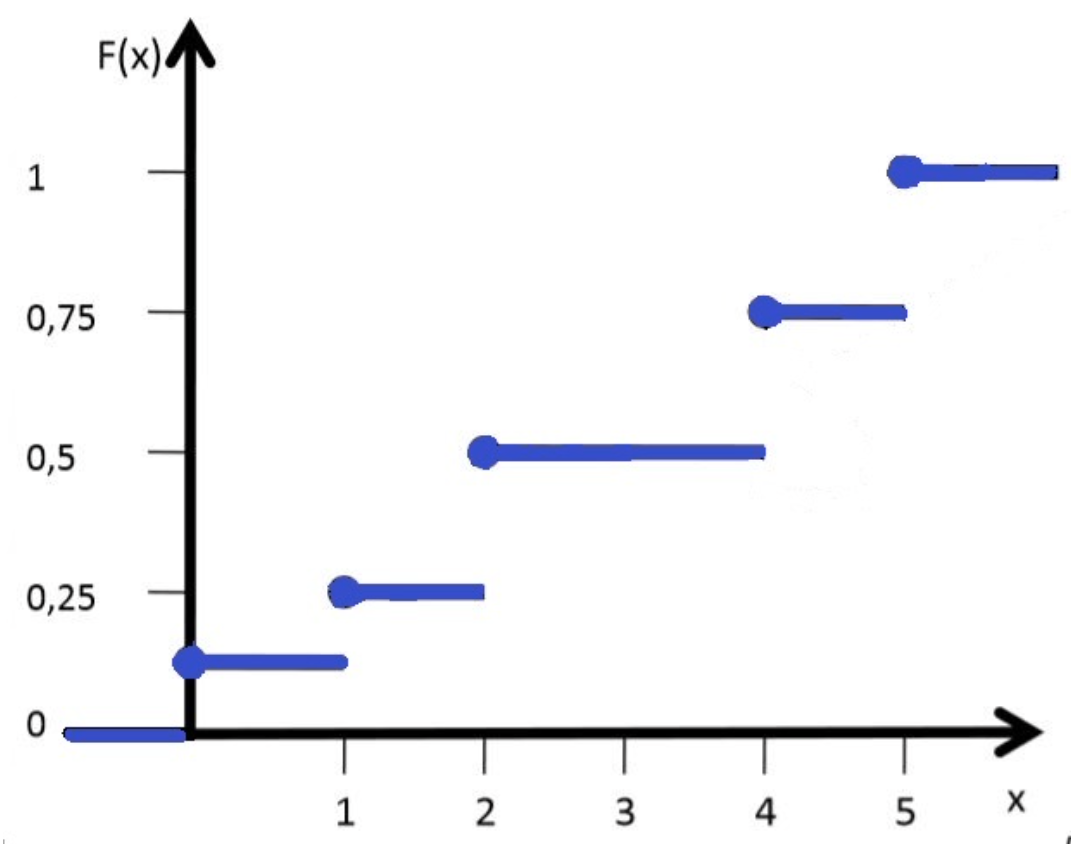
\includegraphics[width=0.3\textwidth]{assets/b03_task3.png}
        \end{center}
    \end{figure}

    \begin{enumerate}
        \item[(a)] Welche Merkmalsausprägungen (verschieden, positiv) wurden für $X$ beobachtet?
    \end{enumerate}
\end{task}

\begin{task}
    \begin{enumerate}
        \item[(b)] Bestimmen Sie die absoluten Häufigkeiten der Merkmalsausprägungen von $X$.
    \end{enumerate}
\end{task}

\begin{task}
    \begin{enumerate}
        \item[(c)] Berechnen Sie das arithmetische Mittel $\overline{x}$ sowie die (korrigierte) Varianz $s^2$ der Daten.
    \end{enumerate}
\end{task}

\begin{task}
    \begin{enumerate}
        \item[(d)] Es wird eine Stichprobe mit zehn weiteren Beobachtungen erhoben. Alle zehn Beobachtungen haben den Wert $3$. Wie lauten dann die neuen relativen Häufigkeiten der Merkmalsausprägungen von $X$ für die um jene Beobachtungswerte erweiterte Stichprobe?
    \end{enumerate}
\end{task}

% !TeX root = ../b01.tex

\section{Aufgabe BI-4}

\begin{task}
    In der Verwaltung einer bestimmten Hochschule sind 400 Personen beschäftigt. Jede Person ist entweder Arbeiter/in, angestellt oder beamtet. Die Aufteilung in Abhängigkeit vom Geschlecht ist in der Kontingenztabelle

    \begin{table}[H]
    \centering
    \begin{tabular}{l|c|c|c}
                 & Arbeiter/in & angestellt & beamtet \\ \hline
        weiblich & 5           & 160        & 42      \\
        männlich & 36          & 122        & 35     
    \end{tabular}
    \end{table}

    zusammengestellt. Bestimmen Sie für jene Daten das Kontingenzmaß $V$ nach Cramér und interpretieren Sie jenen Werte.
\end{task}

% !TeX root = ../b01.tex

\section{Aufgabe BI-5}

\begin{task}
    Eine Gesamtstichprobe von 20 Elementen, bei der man sich für zwei Merkmale $X$ und $Y$ interessiert, wurde zur Datenerhebung in zwei gleich große Teilstichproben aufgeteilt. Für die Teilstichproben ergaben sich dabei die folgenden Maßzahlen:

    \begin{table}[H]
    \centering
    \begin{tabular}{c|cccccc}
        Teilstichprobe $j$ & $n_j$ & $\overline{x}_{n_j}^{(j)}$ & $\overline{y}_{n_j}^{(j)}$ & $\tilde{s}_{X,X}^{(j)}$ & $\tilde{s}_{Y,Y}^{(j)}$ & $r_{X,Y}^{(j)}$ \\ \hline
        1 & 10 & 12 & 0 & 36 & 9  & 1 \\
        2 & 10 & 0  & 6 & 9  & 36 & 1
    \end{tabular}
    \end{table}

    Wie groß ist dann der Korrelationskoeffizient nach Bravais-Pearson $r_{X,Y}$ für die Gesamtstichprobe?
\end{task}

% !TeX root = ../b01.tex

\section{Aufgabe BI-6}

\begin{task}
    Unter 10 Studierenden wurde ein Wettlauf veranstaltet. Die folgende Tabelle enthält die Körpergröße (Merkmal $X$) und die Platzierung (Merkmal $Y$) der 10 Teilnehmer:

    \begin{table}[H]
    \centering
    \begin{tabular}{c|cccccccccc}
        Körpergröße (in cm) & 181 & 171 & 166 & 175 & 183 &191 & 170 & 179 & 185 & 190 \\ \hline
        Platzierung & 3 & 7 & 10 & 8 & 5 & 2 & 9 & 6 & 1 & 4
    \end{tabular}
    \end{table}

    \begin{enumerate}
        \item[(a)] Ermitteln Sie Schätzwerte $\hat{a}$ und $\hat{b}$ für die Parameter $a$ und $b$ aus dem Regressionsmodell $Y=a+bX$ mit
        $a,b\in\mathbb{R}$
        nach der Methode der kleinsten Quadrate.
    \end{enumerate}
\end{task}

\begin{task}
    \begin{enumerate}
        \item[(b)] Berechnen Sie das Bestimmtheitsmaß $R^2$ für das lineare Regressionsmodell gemäß (a) sowie den empirischen Korrelationskoeffizient $r_{X,Y}$ und interpretieren Sie kurz Ihre Ergebnisse.
    \end{enumerate}
\end{task}

\begin{task}
    \begin{enumerate}
        \item[(c)] Bestimmen Sie (zum Vergeich) den Rangkorrelationskoeffizienten $r_{X,Y}^*$ nach Spearman (da ja im Grunde das Merkmal $Y$ nur ordinalskaliert ist) und interpretieren Sie kurz Ihr Ergebnis.
    \end{enumerate}
\end{task}


\end{document}
